\section{Silizium-PVD}
\label{siliconpvd}

Mit Silizium soll ein weiteres PVD-Material untersucht werden, das im Gegensatz zu den bisher untersuchten Metallen, welche ungerichtete Bindungen aufbauen und damit die kristalline Strukturen bevorzugen, auf gerichteten Bindungen beruht.
Deshalb werden reaktive Kraftfelder genutzt, welche Bindungen explizit über Bindungsordnungen benachbarter Atome beschreiben.

Da die ReaxFF-Formulierung erst innerhalb des letzten Jahrzehntes an Popularität gewonnen hat, sind die verfügbaren Parametersätze auf sehr spezielle Probleme angepasst und unterstützen zumeist entweder Bulkmaterialien oder Reaktionen zwischen Molekülen.
Tabelle~\ref{tab:siliconpotentials} listet die im Rahmen der Arbeit untersuchten ReaxFF-Parametrisierungen auf.

\begin{table}[bh]
  \caption{Untersuchte ReaxFF-Parametrisierungen für Silizium- und Siliziumoxidsysteme}
  \label{tab:siliconpotentials}
  \oddrowcolors
  \begin{tabularx}{1\textwidth}{|lXc|}
    \hline
    \textbf{Parametrisierung} & \textbf{Anwendung \& Kommentare}                                                                          & \textbf{Ref.}                     \\
    \hline
    \pot{Al\_Al0\_AlN}        & \ce{Al}, \ce{Al2O3}, \ce{AlN}. Basiert auf einer Si-Parametrisierung                                      & \cite{plimpton_lammps_2014}       \\
    \pot{chenoweth}           & Zersetzung von Polydimethylsiloxane bei hohen Drücken und Temperaturen. Ergänzung von \ce{C-Si}-Bindungen & \cite{chenoweth_simulations_2005} \\
    \pot{kulkarni}            & Reaktion von Sauerstoff mit \ce{OH}-terminiertem Siliziumoxid                                             & \cite{kulkarni_oxygen_2013}       \\
    \pot{lg}                  & ``low gradients''. Siehe liu\_nitramines. Fehlerhafte Version aus LAMMPS\cite{plimpton_lammps_2014}       & \cite{liu_reaxff-lg:_2011}        \\
    \pot{liu\_ettringite}     & Verspannung von Ettringit (\ce{Ca6[Al(OH)6]2(SO4)3 26H2O}). Basiert auf Si-Parametrisierung               & \cite{liu_development_2012}       \\
    \pot{liu\_nitramines}     & Dichtebestimmung von Nitramin-Molekülen bei hohen Drücken. Dichte erhöht durch Van-der-Waals-Korrekturen  & \cite{liu_reaxff-lg:_2011}        \\
    \pot{narayanan}           & Präparation mit \ce{Li-Al}-Silikaten. Für Phasenübergänge von Eukryptit-Kristallen (\ce{LiAl[SiO4]})      & \cite{narayanan_reactive_2012}    \\
    \pot{newsome}             & Oxidation von \ce{SiC}-Oberflächen bei \SIrange{500}{5000}{\kelvin}                                       & \cite{newsome_oxidation_2012}     \\
    \pot{nielson}             & Reaktionskinetik an Metallkatalysatoren bei \SI{1500}{\kelvin}                                            & \cite{nielson_development_2005}   \\
    \pot{zhang}               & Zersetzung energiereicher Moleküle (Nitramin-Explosionen)                                                 & \cite{zhang_carbon_2009}          \\
    \hline
  \end{tabularx}
\end{table}

\subsection{Voruntersuchungen}

Zur Abschätzung der Anwendbarkeit der Parametersätze auf die Simulation von Silizium-PVD wurden die amorphe und kristalline Phase auf Stabilität und strukturelle Eigenschaften geprüft (Tabelle~\ref{tab:siliconpreresults}).
Zusätzlich wurden in Hinblick auf Siliziumoxid-CVD auch die Precursormoleküle Silan und Sauerstoff untersucht, welche nur in Anhang~\ref{appendix_silica} betrachtet werden, da bisher kein vollständiger Abscheidungsprozess simuliert wurde.
Referenzwerte stammen aus den Referenzen~\cite{haynes_crc_2011,remes_optical_1998} und sind in Anhang~\ref{appendix_constants} zusammen gefasst.
\nopagebreak[4]
\begin{table}[th]
  \begin{threeparttable}
    \caption{Zusammenfassung der Ergebnisse der Silizium-Voruntersuchungen}
    \label{tab:siliconpreresults}

    \oddrowcolors
    \begin{tabularx}{\textwidth}{|lCCCCCC|}
      \hline
      \textbf{Parametrisierung} & \textbf{LMP\tnote{a}} & \textbf{c-\ce{Si}} & \textbf{a-\ce{Si}} & \textbf{PVD\tnote{b}} & \ce{SiH4}\tnote{c} & \ce{+O2}\tnote{c} \\
      \hline                %   & LAMMPS                & c-Si               & a-Si               & PVD                   & Silane             & +O2               \\
      \pot{Al\_Al0\_AlN}        & \cmark                & ~                  & \cmark             & \cmark                & \cmark             & ~                 \\
      \pot{chenoweth}           & ~                     & ~                  & ~                  & ~                     & ~                  & ~                 \\
      \pot{kulkarni}            & \cmark                & \cmark             & \cmark             & \cmark                & \cmark             & (\cmark)          \\
      \pot{lg}                  & ~                     & ~                  & ~                  & ~                     & ~                  & ~                 \\
      \pot{liu\_ettringite}     & \cmark                & ~                  & \cmark             & \cmark                & ~                  & ~                 \\
      \pot{liu\_nitramines}     & ~                     & ~                  & ~                  & ~                     & ~                  & ~                 \\
      \pot{narayanan}           & \cmark                & ~                  & \cmark             & \cmark                & ~                  & ~                 \\
      \pot{newsome}             & \cmark                & ~                  & ~                  & \cmark                & ~                  & (\cmark)          \\
      \pot{nielson}             & \cmark                & \cmark             & \cmark             & \cmark                & \cmark             & ~                 \\
      \pot{zhang}               & \cmark                & ~                  & \cmark             & ~                     & \cmark             & \cmark            \\
      \hline
    \end{tabularx}

 %% & c-\ce{SiO2} & CVD\tnote{b}
 %% & c-SiO2      & CVD
 %% & (\cmark)    & \cmark?
 %% & ~           & ~
 %% & \cmark      & \cmark?
 %% & ~           & ~
 %% & \cmark      & \cmark?
 %% & ~           & ~
 %% & \cmark      & \cmark?
 %% & (\cmark)    & \cmark?
 %% & \cmark      & \cmark?
 %% & ~           & ~

    \begin{tablenotes}[para]
      \item[a] LMP: Kompatibilität mit LAMMPS
      \item[b] PVD: a-\ce{Si}-PVD mit Parsivald
      \item[c] Ergebnisse der Precursor-Simulationen befinden sich in Anhang~\ref{appendix_silica}
    \end{tablenotes}
  \end{threeparttable}
\end{table}
\nopagebreak[4]
\subsubsection{Kompatibilität mit der Molekulardynamiksoftware LAMMPS (LMP)}

Einige Potentialdateien sind nicht mit der aktuellen Version der LAMMPS-Bibliothek kompatibel, was sich in harten Abbrüchen des Programmes äußert und sie von weiteren Untersuchungen ausschließt.
Die Parametersätze \pot{chenoweth}, \pot{lg} und \pot{liu\_nitra\-mines} konnten aus diesem Grund nicht für MD-Simulationen genutzt werden.

\subsubsection{Kristalleigenschaften (c-\ce{Si})}

\begin{table}[!b]
  \oddrowcolors
  \caption{Struktur von c-\ce{Si} nach der MD-Relaxierung}
  \label{tab:csiresults}

  \begin{tabularx}{\textwidth}{|llXXlX|}
    \hline
    \textbf{Parametrisierung} & \multicolumn{2}{l}{\textbf{Bindungslänge}}   & \textbf{Struktur} & \textbf{Dichte}    & ~                     \\
    \hline
    \textit{kristallin}       & \SI{2.352}{\angstrom} & ~                    & kristallin        & \SI{2.3296}{\gpcc} & ~                     \\
    \pot{kulkarni}            & \SI{2.303}{\angstrom} & \SI{-2.08}{\percent} & kristallin        & \SI{2.481}{\gpcc}  & \SI{+6.50}{\percent}  \\
    \pot{liu\_ettringite}     & \SI{2.325}{\angstrom} & \SI{-1.15}{\percent} & amorph            & \SI{2.830}{\gpcc}  & \SI{+21.48}{\percent} \\
    \pot{narayanan}           & \SI{2.325}{\angstrom} & \SI{-1.15}{\percent} & amorph            & \SI{2.825}{\gpcc}  & \SI{+21.27}{\percent} \\
    \pot{newsome}             & \SI{2.359}{\angstrom} & \SI{+0.30}{\percent} & (kristallin)      & \SI{2.427}{\gpcc}  & \SI{+4.18}{\percent}  \\
    \pot{nielson}             & \SI{2.293}{\angstrom} & \SI{-2.51}{\percent} & kristallin        & \SI{2.512}{\gpcc}  & \SI{+7.83}{\percent}  \\

%% & \textbf{Koord.}
%% & \num{4.00}
%% & \num{4.00}
%% & \num{4.00}
%% & \num{4.00}
%% & \num{4.00}
%% & \num{4.00}

    \hline
  \end{tabularx}
\end{table}

Eine Parametrisierung gilt als erfolgreich bei der Beschreibung von kristallinem Silizium, wenn bei einer Relaxierung des Kristalles bei \SI{600}{\kelvin} (Schmelztemperatur: \SI{1687}{\kelvin}\cite{haynes_crc_2011}) über \num{100000} Zeitschritte mit anschließender Abkühlung auf \SI{50}{\kelvin} die Gittereigenschaften bewahrt werden.
Dafür werden die Dichten und die aus der radialen Verteilungsfunktion gewonnenen Koordinationszahlen und Bindungslängen mit Referenzwerten\cite{haynes_crc_2011} verglichen (Tabelle~\ref{tab:csiresults}).
Die RDF wird außerdem hinsichtlich der Struktur des Materiales untersucht (Abbildung~\ref{fig:siliconrdf}).

\begin{figure}[p]
  \centering

  \captionsetup[subfigure]{singlelinecheck=false}
  \def\subfigwidth{\textwidth}
  \begin{subfigure}[t]{\subfigwidth}
    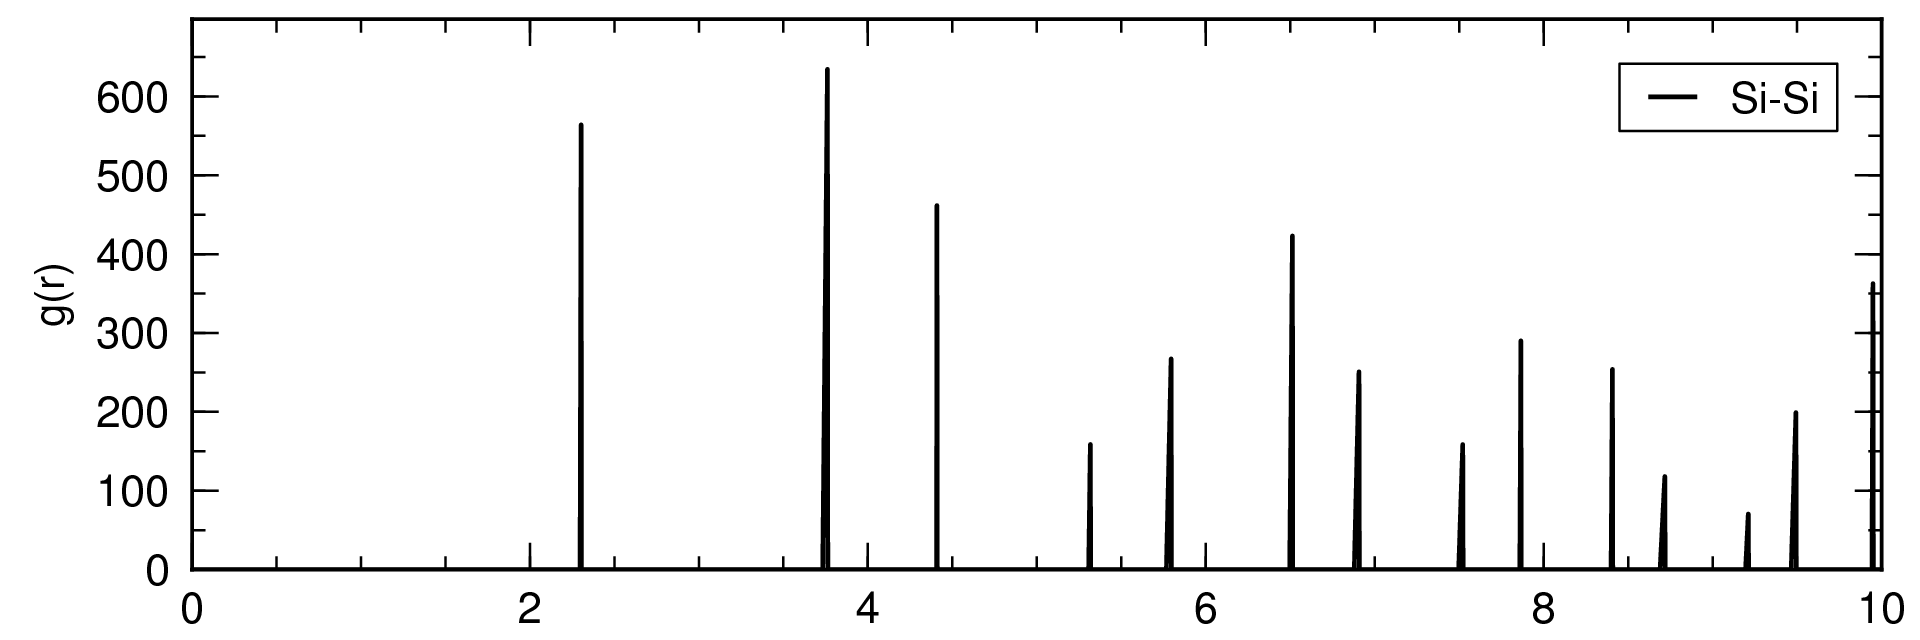
\includegraphics[width=\textwidth]{Si_kulkarni_rdf}
    \subcaption{\pot{kulkarni}: Kristallstruktur mit schmalen, hohen Spitzen in der RDF}
    \label{fig:kulkarnirdf}
  \end{subfigure}

  \vspace{1em}

  \begin{subfigure}[t]{\subfigwidth}
    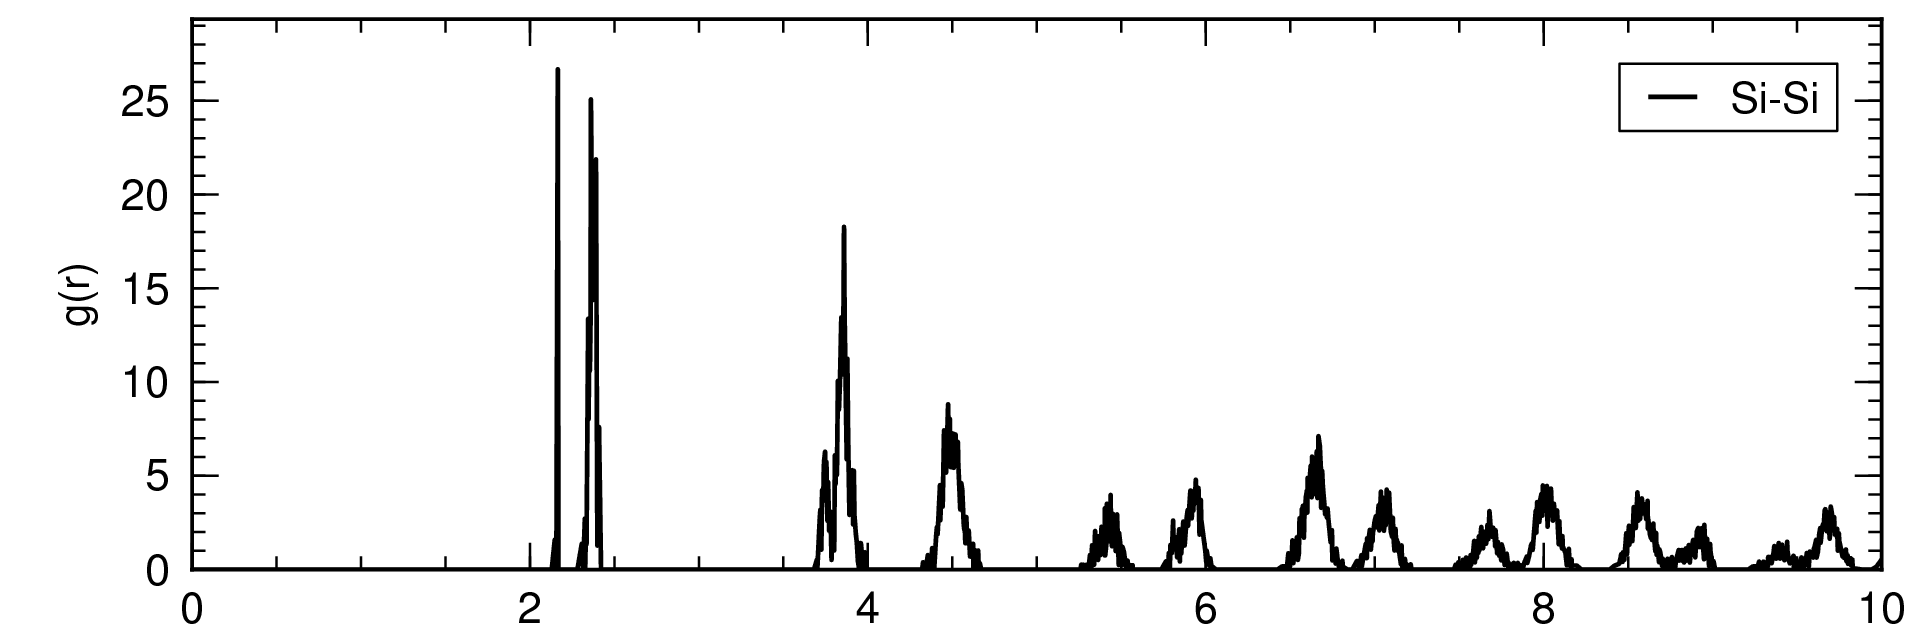
\includegraphics[width=\textwidth]{Si_newsome_rdf}
    \caption{\pot{newsome}: Aufspaltung der Hauptbindungslänge, Kristallstruktur ist noch erkennbar}
    \label{fig:newsomerdf}
  \end{subfigure}

  \vspace{1em}

  \begin{subfigure}[t]{\subfigwidth}
    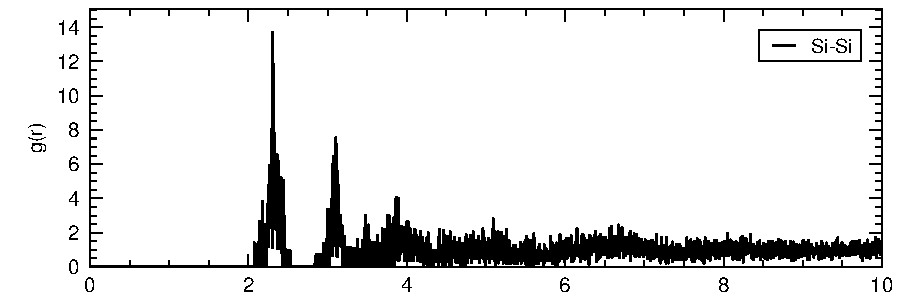
\includegraphics[width=\textwidth]{Si_liu_rdf}
    \caption{\pot{liu\_ettringite}: Verformung zu einer amorphen Struktur ohne langreichweitige Ordnung}
    \label{fig:liurdf}
  \end{subfigure}

  \caption{RDF-Diagramme von c-\ce{Si}-Strukturen nach der MD-Relaxierung}
  \label{fig:siliconrdf}
\end{figure}

Lediglich \pot{kulkarni} und \pot{nielson} sind dabei erfolgreich, wohingegen sich mit \pot{narayanan} und \pot{liu\_ettringite} amorphe Strukturen bilden, was sich auch in der stark überschätzten Dichte zeigt.
\pot{newsome} zeigt zudem in allen Berechnungen eine Aufspaltung der Hauptbindungslänge (Abbildung~\ref{fig:newsomerdf}), welche dadurch in einigen Auswertungen unterschätzt wird.

\subsubsection{Amorphes Silizium (a-\ce{Si})}

Zur Untersuchung amorpher Siliziumstrukturen wurden diese durch Relaxierung zufälliger Siliziumstrukturen mit einer Dichte von \SI{2.11}{\gpcc} im kanonischen Ensemble bei \SI{1500}{\kelvin} erzeugt und auf \SI{50}{\kelvin} abgekühlt, bevor sie mit den oben beschriebenen Methoden analysiert wurden.
Aufgrund der Spannweite möglicher amorpher Strukturen gilt eine Parametrisierung hier allgemein als erfolgreich, wenn sie in einer stabilen Relaxation eine amorphe Struktur erzeugen kann, weshalb beinahe alle Parametrisierungen einen Erfolg vorweisen.

\begin{table}[h]
  \begin{threeparttable}

    \caption{Vergleich der strukturellen Eigenschaften von amorphem Silizium}
    \label{tab:amorphoussilicon}

    \oddrowcolors
    \begin{tabularx}{\textwidth}{|llXXlX|}
      \hline
      \textbf{Parametrisierung} & \multicolumn{2}{l}{\textbf{Bindungslänge}}   & \textbf{Koord.} & \textbf{Dichte}    & ~                        \\
      \hline
      \textit{(kristallin)}     & \SI{2.352}{\angstrom} & ~                    & \num{4.00}      & ~                  & ~                        \\
      \textit{amorph}           & ~                     & ~                    & ~               & \SI{2.29}{\gpcc} \cite{remes_optical_1998} &  \\
      \pot{Al\_Al0\_AlN}        & \SI{2.379}{\angstrom} & \SI{+1.15}{\percent} & \num{4.59}      & \SI{2.373}{\gpcc}  & \SI{+3.62}{\percent}     \\
      \pot{kulkarni}            & \SI{2.339}{\angstrom} & \SI{-0.55}{\percent} & \num{4.05}      & \SI{2.361}{\gpcc}  & \SI{+3.10}{\percent}     \\
      \pot{liu\_ettr.}          & \SI{2.401}{\angstrom} & \SI{+2.08}{\percent} & \num{4.10}      & \SI{2.314}{\gpcc}  & \SI{+1.05}{\percent}     \\
      \pot{narayanan}           & \SI{2.383}{\angstrom} & \SI{+1.32}{\percent} & \num{4.05}      & \SI{2.365}{\gpcc}  & \SI{+3.28}{\percent}     \\
      \pot{newsome}             & \SI{2.153}{\angstrom} & \SI{-8.46}{\percent} & \num{1.17}      & \SI{2.398}{\gpcc}  & \SI{+4.72}{\percent}     \\
      \pot{nielson}             & \SI{2.411}{\angstrom} & \SI{+2.51}{\percent} & \num{4.82}      & \SI{2.358}{\gpcc}  & \SI{+2.97}{\percent}     \\
      \pot{zhang}               & \SI{2.357}{\angstrom} & \SI{+0.21}{\percent} & \num{4.39}      & \SI{2.329}{\gpcc}  & \SI{+1.70}{\percent}     \\
      \hline
    \end{tabularx}

  \end{threeparttable}
\end{table}

\begin{figure}[!b]
  \centering
  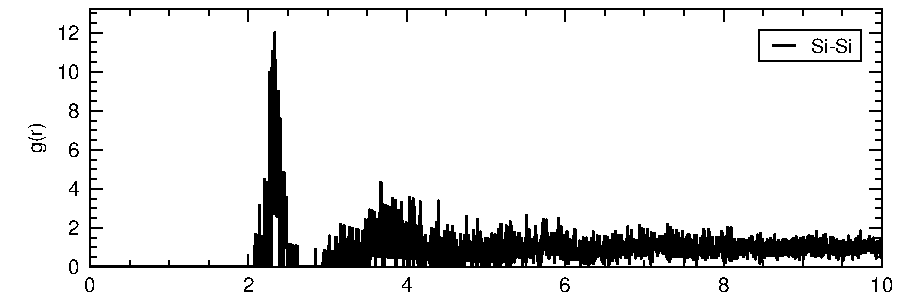
\includegraphics[width=\textwidth]{kulkarni_rdf_amorphous}
  \caption[Radiale Verteilungsfunktionen von relaxiertem a-\ce{Si}]{
    RDF von a-\ce{Si} mit \pot{kulkarni}-Parametrisierung: keine Kristallisation erkennbar
    }
  \label{fig:amorphousrdf}
\end{figure}

Die Ergebnisse dieser Untersuchungen führen zu ähnlichen Ergebnissen für alle Parametersätze (Tabelle~\ref{tab:amorphoussilicon}), wobei \pot{newsome} erneut zur Unterschätzung der Bindungslänge neigt.
Die Bindungslängen sind mit \SI{<3}{\percent} Abweichung in Übereinstimmung mit der Bindungslänge von kristallinem Silizium.
Simulationen mit \pot{kulkarni}, \pot{liu\_ettringite} und \pot{narayanan} zeigen auch eine Koordination von $\approx\num{4}$, die sich aus der Anzahl von Bindungen für Siliziumatome ergibt, doch konnten nicht alle Parametrisierungen diesen Wert reproduzieren.
Somit zeigt sich die ReaxFF-Formulierung bei korrekter Parametrisierung erfolgreich in der Vermeidung von Überkoordinationen.
Bei Untersuchungen der Dichte zeigen alle Parametrisierungen eine systematische Überschätzung des Referenzwertes von \SI{2.29}{\gpcc}\cite{remes_optical_1998} um wenige Prozent, die bereits bei der Untersuchung kristalliner Strukturen beobachtet werden konnte (Tabelle~\ref{tab:csiresults}).
Untersuchungen der RDF-Diagramme zeigt keine langreichweitige Ordnung nach \SI{4}{\angstrom} und somit die Bildung von amorphen Strukturen (exemplarisch Abbildung~\ref{fig:amorphousrdf} für \pot{kulkarni}).

\subsubsection{Abscheidungssimulationen (PVD)}

Die Simulationen von Silizium-PVD selbst verlaufen wie in Kapitel~\ref{parsivald} vorgestellt und unterscheiden sich kaum von den Parsivald-Simulationen der vorherigen Abschnitte.
Durch den Aufbau von gerichteten Bindungen zwischen den Silizium-Atomen wird die Bildung amorpher Schichten erwartet, die sich auch durch verringerte Mobilität der Atome auf der Oberfläche ergibt.
Eine Simulation gilt als erfolgreich, wenn die Parsivald-Simulation erfolgreich terminiert und einen dichten Silizium-Film gebildet hat.
Bis auf die \pot{zhang}-Parametrisierung, bei der sämtliche MD-Simulationen ohne Fehlerausgabe abgestürzt sind, konnten alle Parametrisierungen einen dünnen Film erzeugen.
Aufgrund der insgesamt guten Ergebnisse wurden alle weitergehenden PVD-Simulationen mit dem \pot{kulkarni}-Parametersatz durchgeführt.

\subsubsection{Vorbereitungen chemischer Gasphasenabscheidungen}

Tabelle~\ref{tab:siliconpreresults} zeigt auch Ergebnisse zu Voruntersuchungen der chemischen Gasphasenabscheidungen, die in Anhang~\ref{appendix_silica} kurz vorgestellt werden.
Als Favorit stellt sich hier der \pot{kulkarni}-Parametersatz heraus, der sowohl amorphe und kristalline Strukturen und Oberflächen als auch Moleküle und einige Reaktionen zufriedenstellend beschreiben kann.

\subsection{Simulationen von Silizium-PVD}

Unter Nutzung der \pot{kulkarni}-ReaxFF-Parametrisierung wurden physikalische Abscheidungen dünner Schichten aus amorphem Silizium simuliert.
Als Parameter für die Simulationen wurden $A_\text{sim} = \SI{106x104}{\angstrom}$, $A_\text{MD} = \SI{37x37}{\angstrom}$, $T = \SI{1300}{\kelvin}$, $\Delta t = \SI{10}{\femto\second}$, $\tau = \SI{50}{\femto\second}$, $t_\text{relax} = \SI{3.5}{\pico\second}$ und $E_\text{kin} = \SI{6.2}{\electronvolt}$ genutzt, woraus sich in Messungen $T_\text{MD} = \SI{60.71}{\second}$ und $p = \num{1.68}$ ergeben haben.
Die Temperatur wurde als Kompromiss mit \SI{1300}{\kelvin} bewusst sehr hoch gewählt, um die Relaxierungen zu beschleunigen, da die gesamte Laufzeit bereits \SI{22.5}{\day} beträgt und linear mit der MD-Laufzeit steigt.
Die langen Laufzeiten ergeben sich als Resultat der ReaxFF-Kraftfelder, welche im Vergleich mit anderen Kraftfeldern um ein Vielfaches rechenaufwendiger sind und auch für die mittlere Zahl von \num{1511} Atomen pro Ereignis lange Laufzeiten verursachen.
Deshalb sind mit ihnen aber auch reine MD-Simulationen auf der hier vorgestellten Größenordnung praktisch nicht realisierbar, wobei für Parsivald eine effiziente Größe von $w_\text{eff} = \SI{539}{\nano\meter}$ mit $p_\text{max} = \num{2335}$ bei $\rho_\text{worker} = \SI{11}{\percent}$ berechnet wurde.

Das Ergebnis der Abscheidungssimulation ist eine amorphe Siliziumschicht, die mit konstanter Rate wächst.
Aufgrund von sich langsam verstärkenden Oberflächenunebenheiten nimmt hier die Rauheit beim Wachstum zu (Abbildung~\ref{fig:siliconresults}).
Die Simulationen wurden für die Abscheidungen auf den Kristallebenen (001), (011)- und (111) wiederholt, zeigten aber keine Veränderung der Ergebnisse.
In der RDF der Schicht (Abbildung~\ref{fig:siliconresults-b}) ist das kristalline Substrat in Form von Spitzen erkennbar, doch zeigen sich ansonsten Charakteristika einer amorphen Struktur.

\begin{figure}[t]
  \captionsetup[subfigure]{singlelinecheck=false}
  \def\subfigwidth{0.48\textwidth}
  \begin{subfigure}[t]{\subfigwidth}
    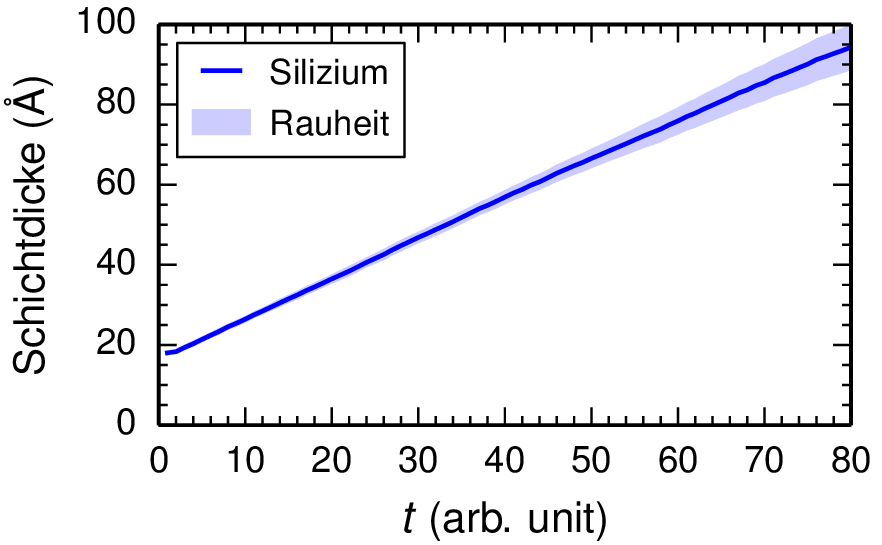
\includegraphics[width=\textwidth]{Si111_combined}
    \subcaption{Dicke und Rauheit der Schicht}
    \label{fig:siliconresults-a}
  \end{subfigure}
  \hfill
  \begin{subfigure}[t]{\subfigwidth}
    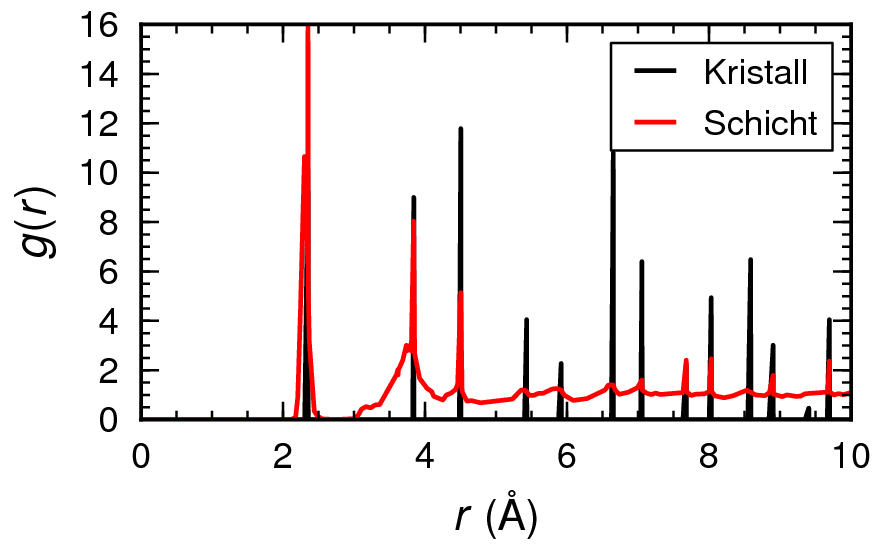
\includegraphics[width=\textwidth]{si111_rdf}
    \subcaption{Radiale Verteilungsfunktion bei $t=80$}
    \label{fig:siliconresults-b}
  \end{subfigure}
  \caption[Struktur einer Silizium-PVD-Schicht aus Parsivald]{
    Struktur einer Silizium-PVD-Schicht aus Parsivald (\SI{10x10x8}{\nano\meter})
  }
  \label{fig:siliconresults}
\end{figure}

Die Unebenheiten der Oberfläche, welche Tiefen von \SI{30}{\angstrom} erreichen können, liegen hauptsächlich in der Form vieler Nanoporen vor, welche eine maximale Breite von wenigen Nanometern haben (Abbildung~\ref{fig:siliconprofile}).
Im Gegensatz zu den Vertiefungen während der Kupfer-PVD (Abschnitt~\ref{copperpvd}) werden diese nicht vollständig mit dem weiteren Wachstum der Schicht geschlossen, sodass die Ausbildung über längere Zeiträume ermöglicht wird.
Die Rauheit der Oberfläche erreicht gegen Ende der Simulation einen RMS-Wert von \SI{1.15}{\nano\meter}, welcher nur um einen Faktor von \num{10} oberhalb der Rauheiten der zuvor betrachteten kristallinen Schichten liegt.
Durch die begrenzte Simulationszeit ist keine Aussage über den weiteren Verlauf der Rauheit möglich, die womöglich in einen sublinearen Verlauf durch Schließung der Unebenheiten übergehen kann.
Es ist ein schwacher Einfluss der Poren auf die Schichtdicke (Abbildung~\ref{fig:siliconresults-a}) erkennbar, welche gegen Ende der Simulation trotz konstanter PVD-Rate sublinear steigt.
Somit wird die Schichtdicke unterschätzt, was sich auch in der höheren Dichte der Struktur von \SI{2.597}{\gpcc} (Referenzen~\cite{remes_optical_1998,renner_density_1973}: \SIrange{2.20}{2.30}{\gpcc}) zeigt.

Zur Untersuchung des Einflusses von Unterrelaxierung wurde eine Abscheidung bei \SI{500}{\kelvin} simuliert (Abbildung~\ref{fig:siliconunderrelaxedprofile}), die realistischen Prozessbedingungen entspricht, aufgrund der kurzen Relaxationszeit aber nicht zur vollständigen Relaxation am Adsorptionsort führt.
Es zeigen sich höhere Rauheiten, feinere Nanoporen und steilere Hänge, die zu einer hohen Porösität der Schicht führen, weshalb zu erwarten ist, dass mit höheren Relaxierungszeiten eine verringerte Porenbildung beobachtet werden kann.

\begin{figure}[h!]
  \centering
  \captionsetup[subfigure]{singlelinecheck=false}
  \begin{subfigure}[t]{8.5cm}
    \begin{overpic}[width=\textwidth]{si111_surface_profile}
      \put(-8,0){\includegraphics{1nmscale}}
    \end{overpic}
  \end{subfigure}
  \begin{subfigure}[t]{2.0cm}
    \def\svgwidth{\textwidth}
    \begin{overpic}[width=0.83cm]{greyhalfscale}
      \put(0,0){\input{img/si111_surface_profile_halfscale.pdf_tex}}
    \end{overpic}
  \end{subfigure}
  \caption[Oberflächenprofil einer Silizium-PVD-Schicht]{
    Oberflächenprofil einer per PVD-Simulation erzeugten Schicht
  }
  \label{fig:siliconprofile}
\end{figure}

\begin{figure}[h!]
  \centering
  \captionsetup[subfigure]{singlelinecheck=false}
  \begin{subfigure}[t]{8.5cm}
    \begin{overpic}[width=\textwidth]{si111_underrelaxed_profile}
      \put(-8,0){\includegraphics{1nmscale}}
    \end{overpic}
  \end{subfigure}
  \begin{subfigure}[t]{2.0cm}
    \def\svgwidth{\textwidth}
    \begin{overpic}[width=0.79cm]{greyscale}
      \put(0,0){\input{img/si111_underrelaxed_profile_scale.pdf_tex}}
    \end{overpic}
  \end{subfigure}
  \caption[Oberflächenprofil einer unterrelaxierten \ce{Si}-Schicht]{
    Oberflächenprofil einer unterrelaxierten \ce{Si}-Schicht, PVD-Simulation
  }
  \label{fig:siliconunderrelaxedprofile}
\end{figure}

\subsection{Fazit}

Nach der Auswahl einer passenden ReaxFF-Parametrisierung aus \num{10} Kandidaten wurde mit ihr die Silizium-PVD auf kristallinen Silizium-Substraten unterschiedlicher Orientierungen simuliert, wobei sich amorphe Schichten mit einer Dicke von \SI{80}{\angstrom} gebildet haben.
Die abschnittsweise linear ansteigende Oberflächenrauheit der aufwachsenden Schicht wird dabei durch die Bildung von Nanoporen mit einer Tiefe von \SI{30}{\angstrom} dominiert, die zumindest teilweise durch eine Unterrelaxation der MD-Boxen verursacht werden, weshalb eine weitergehende Optimierung der Simulationsparameter notwendig ist.
